\documentclass[report.tex]{subfiles}
\begin{document}

This chapter presents the \gls{DSL} Volr. \index{Volr}

Before presenting and specifying the language itself, 
it is beneficial to examine existing work within the
programming and simulation of second and third
generation \glspl{NN}.
Following the existing work, a detailed list of requirements
are provided to accurately scope the \gls{DSL}.
Finally, the implementation of the \gls{DSL} is presented and
accompanied by code and test examples.

\section{Related work}
A vast amount of work has been put into the development of software for simulating
neural networks.
This section covers recent work within the simulation of second and third
generation \glspl{NN}, and extracts relevant findings for use in 
Section \ref{sec:requirements}, covering the requirements of the DSL.

The following list does not claim completeness, due to the fragmented and 
fast-paced nature of the field.
To encompass as many relevant findings as possible, the subsequent
references are based on a number of often-cited sources, primarily based on books
\cite{Bishop2006, Russel2007, Eliasmith2015, Lin2018, Nilsson2009, Pearl1988, Rojas1996, Rumelhart1988}, review papers 
\cite{Schmidhuber2014, Blundell2018, Markram2013, Walter2015, Hunsberger2015},
and articles, which will be referenced below.

\subsection{Second generation}
The perhaps most notable product for this type of networks is the Tensorflow \index{Tensorflow}
framework \cite{Abadi2016}.
Tensorflow is an \gls{API} for the description and execution of directed graph 
structures,
that connects varying activation functions and learning mechanisms through the common abstraction
of tensors \cite{Abadi2015}.
Tensorflow is the result of a large collaboration of multiple companies and organisations, who have
developed a comprehensive library of both code as well as infrastructure and extensive support for hardware acceleration \cite{Abadi2015}.

The primary advantage of Tensorflow \index{Tensorflow} comes from 
its foundation in tensors as a general abstraction, that
can be applied to a wide array of problems \cite{Abadi2016}.
Other frameworks have adapted a similar approach, such as PyTorch \cite{PyTorch2018}, 
scikit-learn \cite{Sklearn2018}, Microsoft Cognitive Toolkit (CNTK) \cite{CNTK2018},
Caffe \cite{Caffe2018} and Theano \cite{Theano2018}.

The frameworks Lasagne and Keras are effectively higher-level abstraction
built on top of Theano and Tensorflow respectively \cite{Lasagne2018, Keras2018}.
They both provide imperative \gls{API}s for constructing models in steps, while
including useful utilities for preprocessing data.

Whereas scikit-learn, CNTK, Tensorflow and Theano target \glspl{NN} in general,
PyTorch and Caffe are frameworks that specifically targets deep \glspl{NN}
\cite{PyTorch2018, Caffe2018}.
However, they all rely on second generation \gls{NN} architecture.

To provide a comparison between them, a number of examples are provided below.
Listing \ref{code:caffe} shows a network with a single fully connected
layer in Caffe, built to recognise handwritten digits from the 
popular MNIST dataset \cite{LeCun1998}.
Caffe is verbose compared to the full network definitions in PyTorch 
(Listing \ref{code:pytorch}), Keras (Listing \ref{code:keras}) and
Lasagne (Listing \ref{code:lasagne}), but provides additional 
configuration options for the setting of weights and biases in 
individual layers.

\lstset{caption={A network layer for the MNIST task in Caffe.},label={code:caffe}}
\begin{lstlisting}
layer {
  name: "ip1"
  type: "InnerProduct"
  param { lr_mult: 1 }
  param { lr_mult: 2 }
  inner_product_param {
    num_output: 500
    weight_filler { type: "xavier" }
    bias_filler { type: "constant" }
  }
  bottom: "pool2"
  top: "ip1"
}
\end{lstlisting}

\lstset{language=Python,caption={MNIST network in PyTorch.},label={code:pytorch}}
\begin{lstlisting}{language=Python}
self.fc1 = nn.Linear(28*28, 128)   # Topology
self.fc2 = nn.Linear(128, 10)
x = x.view(-1, 28, 28)             # Activations
x = F.relu(self.fc1(x))
X = self.fc2(x)
\end{lstlisting}

\lstset{language=Python,caption={MNIST network in Tensorflow using the Keras API.},label={code:keras}}
\begin{lstlisting}
keras.Sequential([
  keras.layers.Flatten(input_shape=(28, 28)),
  keras.layers.Dense(128, activation=tf.nn.relu),
  keras.layers.Dense(10, activation=tf.nn.softmax)
])
\end{lstlisting}

\lstset{language=Python, caption={MNIST network in Theano using the Lasagne API.},label={code:lasagne}}
\begin{lstlisting}
l_in = lasagne.layers.InputLayer(shape=(None, 1, 28, 28),
           input_var=input_var)
l_hid = lasagne.layers.DenseLayer(l_in, num_units=128,
           nonlinearity=lasagne.nonlinearities.rectify)
l_out = lasagne.layers.DenseLayer(
           l_hid, num_units=10,
           nonlinearity=lasagne.nonlinearities.softmax)
\end{lstlisting}

In terms of learning, the frameworks are diverse, although gradient descent 
and auto-differentiation (where transformations are automatically registered and 
later derived using the chain rule) are among the most common features 
(seen in Tensorflow, PyTorch, CNTK, Theano and Caffe). 

Finally, the Open Neural Network Exchange Format (ONNX) is an open data format for the representation
of \gls{ANN} learning models \cite{ONNX2018}. 
ONNX is interesting in this context because, like all the frameworks above, it describes 
networks as directed graphs, defined by nodes of a certain dimension (shape) connected through
edges with certain activations (operations).

\subsubsection{Neural networks in Futhark}
\index{Futhark}
The data-parallel language Futhark is designed to produce efficient parallel
code, suitable for parallel application \cite{Henriksen2017, Elsman2018}.
Futhark is a functional language which operates with higher-order functions as
well as modules \cite{Elsman2018b, Hovgaard2018}.
As argued above, second generation \glspl{NN} can be understood as compositions
of functions, which makes Futhark a suitable language for the implementation of
\glspl{NN}. 

Futhark supports hardware acceleration through the \gls{OpenCL} framework,
and can integrate with other languages, such as \gls{Python} through the
PyOpenCL interface \cite{PyOpenCL}.

\citeauthor{Minh2018} developed a Futhark library for machine learning, which 
allows the construction of densely connected layers and gradient descent
training \cite{Minh2018}.

\subsection{Third generation}
The landscape for third generation software is less homogeneous, which is
primarily due to the fact that the field is still young \cite{Maass1997,
Albada2018}.
Secondly, there are two different approaches to the evaluation of \glspl{SNN}:
through simulation on general purpose hardware or specialised analogue
(neuromorphic\index{neuromorphic}) hardware \cite{Maass1997, Davison2009, Albada2018}.

For each platform --- digital or otherwise --- a complete programming environment
is developed from scratch, because of the degree of specialisation
\cite{Walter2015, Lin2018}.
This section covers the most important technical details of
the environments.

\subsubsection{\Gls{SNN} simulators} \label{sec:SNN-simulators}
Based on the review of \textcite{Blundell2018}, this paper will discuss
the following third generation \gls{SNN} simulators: PyNN \cite{Davison2009},
NEST \cite{Gewaltig2007}, NEURON \cite{Carnevale2007},
Brian \cite{Goodman2013} and Nengo \cite{Eliasmith2015}.

PyNN is a ``simulator-independent language''
\cite{PyNN2018} that compiles to both simulated and
accelerated architectures \cite{Davison2009}.
Technically PyNN is not a simulator but acts as an interface to any third generation
backend \cite{Davison2009}.
PyNN currently interfaces with Brian, NEST, BrainScaleS and SpiNNaker
\index{Brian}\index{NEST}\index{BrainScaleS}\index{SpiNNaker}
and is more than 10 years old \cite{Davison2009}, older
than most neuromorphic chips. 
Their \gls{API}s were designed a priori and lacked a number of crucial
elements, which the hardware designers sought
to resolve by augmenting the interface \cite{Pfeil2013, PyNN2018}.
The result is a fragmented environment that supports basic morphologies, 
in which each experiment requires retrofitting to execute correctly on the respective backend \cite{PyNN2018}.

Nengo is a neural simulation environment for large-scale neural models, with
a focus on graphical modelling \cite{Eliasmith2015}. 
The Nengo project is based on the Neural Engineering Framework (NEF)
\index{Neural Engineering Framework} that offers a concise language for
describing third generation simulations \cite{Bekolay2014}, along with
the limited rendering of logical computations (such as logical gates and basic
mathematical functions) into approximated
\gls{NN} structures \cite{Eliasmith2004, Eliasmith2015}.
Nengo supports a wide range of backends---non-spiking networks through Tensorflow,
simulated spiking networks through its custom \gls{OpenCL} engine and 
hardware accelerated networks through the neuromorphic platform SpiNNaker---
but has a limited repertoire of models compared to other simulators
\cite{Nengo2018}.

Listings \ref{code:Nengo} and \ref{code:PyNN} shows how
basic spiking models are defined using Nengo and PyNN.

\begin{minipage}{\linewidth}
\lstset{caption={A simple LIF MNIST population network in Nengo.}, label=code:Nengo}
\begin{lstlisting}
pop_1 = nengo.Ensemble(nengo.LIF(100), 2)
pop_2 = nengo.Ensemble(nengo.LIF(10),  1)
nengo.Connection(pop_1, pop_2)
\end{lstlisting}
\end{minipage}

\begin{minipage}{\linewidth}
\lstset{caption={A simple LIF MNIST network in PyNN.}, label=code:PyNN}
\begin{lstlisting}
pop_1 = nest.Create('iaf_exp_cond', 100)
pop_2 = nest.Create('iaf_exp_cond',  10)
nest.Connect(pop_1, pop_2, 'all_to_all')
\end{lstlisting} 
\end{minipage}
\\[0.3cm]
PyNN and Nengo both attempt to converge platform differences into one single \gls{API}, and
offer high-level description of networks with support for detailed 
configuration.
Nengo also offers an approximated model that can be evaluated in Tensorflow
\cite{Hunsberger2015}, but it does not translate to other simulators like PyNN:
models written for one simulator cannot be transferred to another \cite{Nengo2018}.

The NEST simulator supports both point neurons \index{neuron!point}
and compartmentalised models to support speed as well as sophisticated neuron
geometry \cite{Gewaltig2007}.
NEST claims to focus on ``dynamics, size and structure rather than on the detailed
morphological and biophysical properties of individual neurons''
\cite{Gewaltig2007}.
It has modelled a large number of neuron models and optimisations
\cite{Blundell2018}.

NEURON targets complex and detailed simulations of multi-chamber models, and
attempts to model all aspects of the biophysical properties \cite{Carnevale2007}.
Brian can be located somewhere between NEST and NEURON in terms of adaptability and flexibility because it allows users to
inject their own models through custom equations in plain text \cite{Goodman2013}.

\textcite{Rueckauer2017} implemented a ``Spiking neural network conversion
toolbox'' that converts second generation \glspl{NN} into \glspl{SNN}.
As shown in Section \ref{sec:coding} they approach this by estimating the 
firing rate of LIF \index{LIF} neurons through fixed current inputs,
assuming even Poisson\index{Poisson distribution} distributed signals
throughout the network \cite{Rueckauer2017}.

\subsubsection{Neuromorphic hardware} \label{sec:similar-neuromorphic}
Based on the review of \textcite{Walter2015} and the work from
\textcite{Lin2018}, the following section classifies neuromorphic hardware into
two categories: either as digital interpretations of neural components, 
or as analogue emulations of neural tissue.

Digital neuromorphic chips digitise neural signals and mimic neuron
behaviour either through the regular \gls{vonNeumann}, or
via custom digital components \cite{Walter2015}.
SpiNNaker is an example of the former, where a number of \gls{ARM}
processors are equipped with controllers for handling timers and
interrupts \cite{Walter2015}.
This permits SpiNNaker to compute arbitrary logic, while retaining
a large degree of parallelism \cite{Albada2018}.
IBM's TrueNorth \index{IBM!TrueNorth} and Intel's Loihi \index{Intel!Loihi}
are examples of neuromorphic hardware with custom digital components 
\cite{Walter2015, Lin2018}.
TrueNorth consist of 4096 independently operating neurosynaptic cores, each implementing 256
digital neurons in silicon \cite{Walter2015, ArtificialBrains2018}.
The Loihi seems similar to the TrueNorth chip, with the difference that
its 128 neuromorphic cores feature programmable
synaptic learning rules \cite{Lin2018}.

Analogue neuromorphic chips construct circuits that equal those of biological
neurons \cite{Walter2015}.
BrainScaleS \cite{Schmitt2017}, Neurogrid \cite{BrainsInSilicon2018}, 
and ROLLS (Reconfigurable On-line Learning Spiking)
\cite{Walter2015} are examples of such chips.

BrainScaleS is built on the High Input Count Analog Neural Network (HICANN)
chip, that contains up to 512 neurons depending on the hardware configuration 
\cite{Pfeil2013}.
Several HICANN chips can be integrated to allow the simulation of larger
networks, where dedicated \gls{FPGA}s set weights for each neuron and
communicate with other \gls{FPGA}s on chip \cite{Walter2015}. 
Neurogrid models around $10^6$ two-compartment neurons, where the dendritic
tree is separated from the neuron `soma' \cite{Walter2015}.
The spikes are transmitted digitally through \gls{RAM} \cite{Walter2015}.
The ROLLS processor consists of 256 analogue silicon neurons with
$\sim1.3 \cdot 10^5$ synapses, but with fixed synaptic weights
\cite{Walter2015}.

\section{DSL requirements} \label{sec:requirements}
This section elaborates on four functional requirements for a \gls{DSL} that will allow the testing of the thesis hypothesis.
The requirements steer the specification as defined in Section 
\ref{sec:volr} and later the implementation details in Section
\ref{sec:implementation}.

\paragraph{1. Semantic consistency}
The overarching goal of the \gls{DSL} is to allow the translation 
of \gls{NN} descriptions into semantically similar models in backend runtime
environments.
In other words, a network described in the \gls{DSL} should carry
the same semantic structure when translated to second or third generation
implementations. 

Because of the diverse and incompatible nature of the spiking neural network
landscape, this is non-trivial but necessary if the models are to be
validated across \gls{NN} paradigms.
This requirement is approached empirically, by illustrating examples in
both generations and validate whether they achieved the desired degree
of external validity.

\paragraph{2. Translation to second and third generation}
A second requirement is the translation of the \gls{DSL} into
two runtime environments to permit a sufficient degree of
generalisation.
It is required that the DSL can translate code that evaluate networks
in second generation, simulated third generation, as well as
analog third generation (neuromorphic).

\paragraph{3. Learning}
It is furthermore required that the \gls{DSL} supports a form of
learning, to illustrate the expected theoretical adaptation.
For this purpose, supervised learning through backpropagation\index{backpropagation}
is sufficient for the purpose of this thesis.

\paragraph{4. Well-typed}
As a final functional requirement, the \gls{DSL} is designed to ensure
consistency and disallow any networks that are not well-formed at
compile time.
\\[0.4cm]
\noindent
None of the above mentioned environments fulfil all four requirements.
Models built in Nengo and PyNN\index{Nengo}\index{PyNN} can be evaluated
in both second and third generation environments, but Nengo does not 
offer consistent semantics between the backends and PyNN only allows
for a partial translation into the neuromorphic platforms.
However, PyNN supports a consistent \gls{API} to describe models that, at
least topologically, translate to both simulated and accelerated 
backends.

The following two sections will present the design and implementation of
Volr, while drawing on the requirements above to assess whether and
how they are met.

\section{DSL specification} \label{sec:volr}
\documentclass{report.tex}{subfiles}
\begin{document}
Before diving into the actual experiment built to test the hypothesis, this
chapter discusses and describes the method employed to model spiking
and artificial \gls{NN}s.

Both types of network are architecturally similar, and both are conceived from
the same physiological principles \autocite{dayan2001, russel2007, Nilsson2009, schmidhuber2014}.
The implementations, however, vary greatly.

To ensure internal and external validity in and between the two network types,
it is desirable that the models are as closely related from a theoretical and
practical perspective as possible.
Additionally, to test the hypothesis, it is required that both the artificial
and spiking models can be simulated on regular machine architecture, while
the spiking model requires a neuromorphic hardware platform.

An optimal approach would be to find a tool that leverages the similarities
of the network types, while integrating with the diverse simulated or emulated
targets.
That is, an abstract model of neural networks that can translate into
heterogeneous back-ends, while retaining a high degree of inter-model validity.

A number of general frameworks for artificial neural networks
exist\footnote{
  Among others, see \autocite{ONNX2018}, \autocite{PyTorch2018}, \autocite{TensorFlow2018},
  \autocite{Keras2018} and DyNet \autocite{Neubig2017}.
}, but none of them extend to the spiking domain.
Conversely a number of choices exist for neuromorphic modelling\footnote{
  %TODO: Find sources on internal IBM/Intel stuff
}, but they exclusively evaluate to neuromorphic or spiking neural network
backends \autocite{Jordan2018}.

A domain-specific language (DSL) called Volr was recently presented to
construct reproducible \gls{NN} experiments
\autocite{Pedersen2018:volr}.
The DSL allows the modelling of sufficiently complicated models for
the purpose of this thesis, while providing a set of tools that permits the
model be sent and evaluated on both \gls{ANN} and \gls{SNN} targets.

Some work was required to fully support learning mechanisms on
neuromorphic hardware, and the DSL, as well as the tooling around it, has been
extended for the purpose of this thesis (see appendix \ref{appendix:volr})
The following section describes the grammar and anatomy of Volr in detail.

\section{Volr}
Volr is a declarative DSL designed to model \gls{NN} that seeks a
trade-off between complete, but verbose, descriptions of small
networks and more general designs of large and complex networks.
By separating the network topologies from the detailed physiological properties
of each neuron or neuron population, the language aims to allow simple
experiments with few, concise declarations, as well as larger and more
complicated experiments while retaining readability.

Figure \ref{fig:volr-expr} shows the BNF form of expressions, values and types
in Volr, while figure \ref{fig:volr-rules} lists evaluation rules to apply
when evaluating the expressions.
Finally the \ref{fig:volr-examples} shows an example network that solves
a rudimentary maze task.
% Expressions, evaluation rules and examples
% Expression figure
\begin{figure}
  \begin{tabular}[t]{l l}
    expressions 
    & \texttt{$e$ ::= $n$} \\
    & \begin{minipage}{0.6\textwidth}
      \begin{Verbatim}[mathescape,commandchars=\\\{\}]
    | \textbf{stim} $n$
    | \textbf{pop} $n\ m$
    | \textbf{tar} $n$
    | $e \otimes e$
    | \textbf{let} $x = e$ \textbf{in} $e'$
      \end{Verbatim} 
    \end{minipage} \\
    & \\ % Empty space
    values
    & \texttt{$v$ ::= $n$} \\
    & \\ % Empty space

    types
    & \texttt{$\tau$ ::= \textbf{group} $n\ m$ | \textbf{stimt} $n$ | \textbf{int} }
  \end{tabular}

  \caption{Expressions, values and types of the Volr language.}
  \label{fig:volr-expr}
\end{figure}

\begin{figure}
\begin{prooftree}
  \AxiomC{}
  \RightLabel{\hskip10pt($e1$)}
  \UnaryInfC{$\Gamma \vdash n : \mathbf{int}$}
\end{prooftree}
\begin{prooftree}
  \AxiomC{}
  \RightLabel{\hskip10pt($e2$)}
  \UnaryInfC{$\Gamma \vdash \mathbf{stim}\ n : \mathbf{net}\ 1\ n$}
\end{prooftree}
\begin{prooftree}
  \AxiomC{}
  \RightLabel{\hskip10pt($e3$)}
  \UnaryInfC{$\Gamma \vdash \mathbf{pop}\ n : \mathbf{net}\ 1\ n$}
\end{prooftree}
\begin{prooftree}
  \AxiomC{$\Gamma (x) = \tau$}
  \RightLabel{\hskip10pt($e4$)}
  \UnaryInfC{$\Gamma \vdash x : \tau$}
\end{prooftree}
\begin{prooftree}
  \AxiomC{$\Gamma \vdash e_1 : \mathbf{net}\ l\ m$}
  \AxiomC{$\Gamma \vdash e_2 : \mathbf{net}\ n\ q$}
  \AxiomC{$\Gamma \vdash w : \mathbf{float}$}
  \RightLabel{\hskip10pt($e5$)}
  \TrinaryInfC{$\Gamma \vdash \otimes\ e_1\ e_2\ w : \mathbf{net}\ l\ q$}
\end{prooftree}
\begin{prooftree}
  \AxiomC{$\Gamma \vdash e_1 : \mathbf{net}\ l\ m$}
  \AxiomC{$\Gamma \vdash e_2 : \mathbf{net}\ m\ n$}
  \AxiomC{$\Gamma \vdash w : \mathbf{float}$}
  \RightLabel{\hskip10pt($e6$)}
  \TrinaryInfC{$\Gamma \vdash \ominus\ e_1\ e_2\ w : \mathbf{net}\ l\ n$}
\end{prooftree}
\begin{prooftree}
  \AxiomC{$\Gamma \vdash e : \tau$}
  \AxiomC{$\Gamma [v : \tau] \vdash e' : \tau$}
  \RightLabel{\hskip10pt($e7$)}
  \BinaryInfC{$\Gamma \vdash \mathbf{let}\ x = e\ in\ e' : \tau$}
\end{prooftree}

  \caption{Evaluation rules in Volr.}
  \label{fig:volr-rules}
\end{figure}



\begin{figure}
  \ContinuedFloat*
  \begin{tabular}[t]{l c}
    \begin{minipage}{0.4\textwidth}
      \begin{Verbatim}[mathescape,commandchars=\\\{\}]
\textbf{dense} 2 2
      \end{Verbatim}
    \end{minipage} & \begin{minipage}{0.4\textwidth}
      \includegraphics[width=\textwidth]{chapters/volr/example2.pdf}
    \end{minipage}

  \end{tabular}
  \caption{A network with a stimulus containing two channels.
    The stimulus is fully connected to a population with an excitatory
    weight of 1. Each circular node represents a single neuron.}
  \label{fig:volr-example1}
\end{figure}

\begin{figure}
  \ContinuedFloat
  \begin{tabular}[t]{l c}
    \begin{minipage}{0.4\textwidth}
      \begin{Verbatim}[mathescape,commandchars=\\\{\}]
\textbf{let} s$_1$ = \textbf{dense} 1 1 \textbf{in}
\textbf{let} s$_2$ = $\neg$ \textbf{dense} 1 1 \textbf{in}
(s$_1$ $\ominus$ s$_2$) $\obar$ \textbf{dense} 2 1
      \end{Verbatim}
    \end{minipage} & \begin{minipage}{0.6\textwidth}
      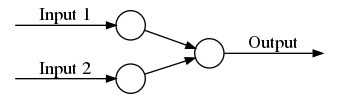
\includegraphics[width=\textwidth]{chapters/volr/example1.pdf}
    \end{minipage}
  \end{tabular}
  \caption{An illustration of a simple binary network, whose two 
	   parallel layers share the middle population of size 2.}
\end{figure}

\begin{figure}
  \ContinuedFloat
  \begin{tabular}[t]{l c}
    \begin{minipage}[b]{0.4\textwidth}
      \begin{Verbatim}[mathescape,commandchars=\\\{\}]
      \textbf{dense} 100 50
        $\obar$ \textbf{dense} 50 10
      \end{Verbatim}
    \end{minipage} & \begin{minipage}{0.5\textwidth}
      \includegraphics[width=\textwidth]{chapters/volr/example3.pdf}
    \end{minipage}
  \end{tabular}
  \caption{A larger network that can process the MNIST dataset
    as 10x10 pixel images. 
    The nodes are populations of neurons,
    where the input corresponds to the pixel size ($10\cdot10=100$) 
    and the output to the possible classes (0 - 9).
    Input and output are implicit.}
\end{figure}

\begin{figure}
  \begin{tabular}[t]{l c}
    \begin{minipage}{0.45\textwidth}
      \begin{Verbatim}[mathescape,commandchars=\\\{\}]
\textbf{let} s = \textbf{dense} 2 2 \textbf{in}
\textbf{let} l$_1$ = \textbf{dense} 2 4 \textbf{in}
\textbf{let} l$_2$ = \textbf{dense} 2 4 \textbf{in}
\textbf{let} o = \textbf{dense} 8 1 \textbf{in} 
  s $\obar$ (l$_1$ $\ominus$ l$_2$) $\obar$ o
      \end{Verbatim}
    \end{minipage} & \begin{minipage}{0.5\textwidth}
       \includegraphics[width=\textwidth]{chapters/volr/example4.pdf}
    \end{minipage}
  \end{tabular}
   \caption{An example where a two-dimensional input is split into
     two nodes and later merged into a node of a single neuron.}
  \label{fig:volr-examples}
\end{figure}



\newpage\null\thispagestyle{empty}\newpage
\newpage\null\thispagestyle{empty}\newpage
\pagebreak
Figure \ref{fig:volr-bnf} shows the constituent parts of an experiment.
Four sub-com\-po\-nents are required:
  A number of stimuli, neural populations, responses and experiment targets.

\subsubsection{Block grammar} \label{sec:volr-block}
The sub-components are constructed using the same declarative \textit{block}
structure shown in figure \ref{fig:volr-ebnf-block}.
The block defines its \textit{type} (\texttt{stimulus}, \texttt{population},
\texttt{response} or \texttt{target}), an optional \textit{name} and lastly
some block content.

The content varies for the different block types, but is restricted to contain
a number of either key-value pairs (\texttt{field}s) or relations to other
blocks (\texttt{connection}s).
Fields are interpreted by the respective targets (see section
\ref{sec:volr-targets}) and connections are only allowed for
\texttt{population}s and \texttt{responses}.

\subsubsection{Connection-set algebra grammar} \label{sec:volr-csa}
Connections between blocks are implemented as a subset of the \gls{CSA}
introduced in section \ref{sec:CSA} \autocite{Djurfeldt2012}.
Most notably, the notion of \textit{blocks} and \textit{geometric distance} have
been omitted\footnote{Neither blocks nor distances are required for the
  experiment in the thesis. It is, however, a necessary element to conduct
  further experiments, since biological \gls{SNN} are highly influenced by
  spatial arrangements \autocite{dayan2001}.
}.

The grammar is presented in figure \ref{fig:volr-ebnf-csa}, and aims to provide
a flexible way to describe complex connectivity patterns in text.
The present grammar can be viewed as a basic algebraic tool for set operations.
Describing full connectivity between two populations, such that all neurons
in the first population is connected with all neurons in the second population,
can simply be expressed as `\texttt{all}'.
Connecting one neuron to one other neuron between two populations are described
as `\texttt{one}', while random connectivity are described with a probability
of, say 0.5: `\texttt{random 0.5}'\footnote{
  This expresses a Bernouilli trial with the given probability
  \autocite{Djurfeldt2012}.
}
As a final example, every neuron in a population connected to every neuron in
that same population, with the exception of identical neurons, can be described
as `\texttt{all - self}'.
%
% \begin{figure}
%   \begin{center}
%     \begin{minipage}{0.8\linewidth}
%       \begin{grammar}
%         <connection> ::= 'from' , <block-name> , { <csa-expr> } ;
%
%         <csa-expr> ::= <csa-term> | <csa-expr> , <csa-operator> , <csa-expr> ;
%
%         <csa-term> ::= 'all' | 'one' | 'self' | 'random' , <number> ;
%
%         <csa-operator> ::= '+' | '-' | '*' ;
%       \end{grammar}
%     \end{minipage}
%   \end{center}
%   \caption{BNF of the connection grammar, describing relations between
%     blocks through \gls{CSA}.}
%   \label{fig:volr-bnf-csa}
% \end{figure}

\subsubsection{Experiment stimuli}
The stimuli describes the ``input'' of the model.
Such input is defined either as an array of elements directly in the DSL
or as a reference to a file.

\subsubsection{Experiment populations}
The populations describe the topology of the neural network itself.
As with the stimuli, the populations are built around a block structure that
contains a number of sub-expressions.

The \texttt{connection} defines the source stimulus for the population,
i.e. the population \textit{from} which action-potentials will be forwarded.
A population can receive stimulus from more than one source.
The connections are modelled as per the \gls{CSA} described in section
\ref{sec:volr-csa}.

% TODO: Describe and invent archetypes... or not?

\subsubsection{Experiment responses}
The responses are the ``output'' of the model to be recorded, and can be
considered as the outcome of the network for training purposes.
The response block only contains an optional specification of a location for
the experiment output data.

\subsubsection{Experiment targets}
The final element in a Volr experiment is its targets.
A target describe a destination environments on which to run the experiment.
These are described in detail in section \ref{sec:volr-targets}, and are
referenced in the grammar as simple strings.

\subsection{Volr semantics}
In practice a network is built by describing a graph.
The nodes in the graph consist of \texttt{populations} of neurons and the edges
are connection-set matrices to other populations \autocite{Djurfeldt2012}.
% TODO: Describe CSA
\texttt{Populations} can consist of any positive number of neurons and is
required to have at least one connection.
Connections can be recursive, resulting in a potentially cyclic graph.
Both the connections and the \texttt{populations} can be annotated with features
such as connection weight and neuron parameters (see \nameref{appendix:volr}).
The parameters are treated differently depending on the experiment target (see
sections \ref{sec:volr-NEST} and \ref{sec:volr-BrainScaleS}).


\section{Neural network simulation targets in Volr} \label{sec:volr-targets}

% TODO :Write how fields are interpreted
% TODO: Write how input is interpreted

Volr exploits the structural similarities between \gls{ANN} and \gls{SNN} to
translate the model to both spiking and artificial network platforms (back-ends).

In the remainder of the chapter the three emulation back-ends, shown in figure
\ref{fig:volr}, are described:
a machine learning target for \gls{ANN}s and a neuron simulation target, as well
as a neuromorphic hardware target, for \gls{SNN}s.

\begin{figure}
  \centering
  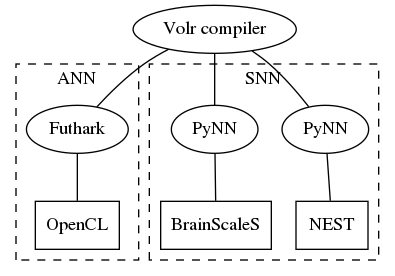
\includegraphics[width=0.6\textwidth]{images/volr-architecture.png}
  \caption{The translation from the Volr DSL to \gls{ANN} simulations in OpenCL via
    \gls{Futhark} and to \gls{SNN} simulations on \gls{NEST} and \gls{BrainScaleS}
    via the \gls{Myelin} middleware.
  }
  \label{fig:volr}
\end{figure}

\subsection{Translation to Futhark} \label{sec:volr-futhark}
Futhark is a functional data-parallel programming language \autocite{Henriksen2017}.
It offers a number of compilation targets such as \gls{OpenCL}, which is
particularly interesting for this thesis because of its capacity for hardware
acceleration.

The practical translation from the Volr model to Futhark is built on recurrent
\gls{ANN} with stochastic gradient descent backpropagation
\autocite{russel2007, schmidhuber2014}.
Each neuron population is considered as a single layer, whose connections are
determined by a connection matrix.

% Deal with recurrent connections
% Describe how this relates to layers

... To be continued ...

\subsection{Spiking neural network simulations via PyNN} \label{sec:volr-pynn}
The Python neural network simulation interface PyNN is designed as a
"simulator-independent language for building neuronal network models"
\autocite{PyNN2018}.
It aims to reduce the problem of diverse, and occasionally unique, descriptions
of neural network experiments for different simulation back-ends \autocite{Davison2009}.
PyNN has been adapted by a number of simulators, including the NEST simulation
platform and the neuromorphic BrainScaleS wafer system
\autocite{Davison2009, Helias2012, Schmitt2017}.

There are still simulator-dependent configurations that seems unlikely to be
adopted into PyNN in the immediate future\footnote{
  Particularly hardware mapping configurations are hard to abstract in a general
  interface.
}.
For that reason Volr provides simulation-specific PyNN scripts that can
interpret the model in the context of each simulation target.
A middleware, dubbed \gls{Myelin}, was invented to translate the \gls{NN} model
into a static intermediate representation in JSON.
The JSON standard was chosen for the task because of its concise syntax while
still retaining human readability.

The advantage of the static experiment representation being, that the experiment
easily a) transports to the target PyNN scripts without losing any information,
and b) duplexes between several experiment; the same experiment setup is
trivial to setup on multiple targets at once.

The correct execution of the experiments relies on the PyNN scripts to exploit
the simulator to represent the Volr model as accurately as possible.
Fortunately PyNN is designed to cover exactly such a use case, so properties
related to the \gls{NN} models itself (such as network topology and population
attributes) were faithfully reproduced across the simulators.
However, the simulators deviate in a number of ways that are relevant to
mention.
The following two sections explains the steps necessary to achieve accurate
experiment environments in \gls{NEST} and \gls{BrainScaleS}.

\subsubsection{Translation to PyNN} \label{sec:volr-translation}

\subsubsection{Translation to NEST} \label{sec:volr-NEST}
... To be continued ...
\subsubsection{Translation to BrainScaleS} \label{sec:volr-BrainScaleS}
... To be continued ...
\end{document}

\section{DSL implementation} \label{sec:implementation}
The compiler for the \gls{DSL} is implemented in the functional language
Haskell \cite{Haskell}.
Currently, Volr translates its network models into two runtime
environments (backends) based on \gls{OpenCL} through Futhark\index{Futhark} and
\glspl{SNN} simulations through PyNN and NEST.\index{PyNN}\index{NEST}
However, using the learning-to-learn paradigm above, the PyNN implementations
opens for the possibility to transfer the optimised models into neuromorphic
hardware such as BrainScaleS\index{BrainScaleS}.

Futhark was chosen because it is concise and offers
useful abstractions that cleanly compose functional
models \cite{Henriksen2017}.
Considering \glspl{NN} as a structure of feedforward and feedback functions,
Futhark is an elegant solution for the task.

PyNN was chosen for its general purpose API that translates to NEST, but also
supports translation into neuromorphic platforms like BrainScaleS. \index{BrainScaleS} 
\index{NEST}
\\[0.2cm]
Figure \ref{fig:volr-architecture} shows the workflow starting with the
compilation of the network model, down to the runtime evaluation on each backend.
The following section explains the diagram one component at a time.

\begin{figure}
  \centering
  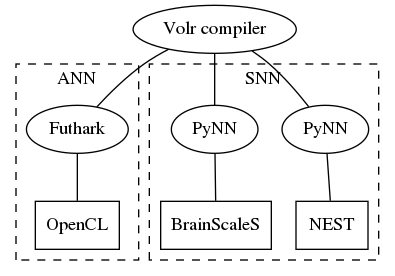
\includegraphics[width=0.4\textwidth]{images/volr-architecture.png}
  \caption{The workflow from the Volr compiler to 
    \gls{ANN} simulations in Futhark and \gls{SNN} simulations in NEST.
  }
  \label{fig:volr-architecture}
\end{figure}

\subsection{The DSL compiler}
The Haskell compiler consists of five different parts:
An \gls{AST}, an evaluator, a language parser and two
code generators for \glspl{ANN} and \glspl{SNN}.

\lstset{mathescape=false,showstringspaces=false}
\begin{minipage}{\linewidth}
  \begin{lstlisting}[language=haskell, caption={The Volr AST in
  Haskell},label={code:term}]
data Term
  = TmNet Int 
  | TmPar Term Term
  | TmSeq Term Term
  | TmRef String
  | TmLet String Term Term
  deriving (Eq, Show)  
\end{lstlisting}
\end{minipage}

The AST reflects the expressions given in the 
specification (see Section \ref{sec:volr}) and is
shown in Listing \ref{code:term}.
It is accompanied by a simple type system (in Listing \ref{code:type})
that similarly maps to the types given above.

\begin{lstlisting}[language=haskell,label={code:type},caption={Volr type system
in Haskell}]
data Type 
  = TyNetwork Int Int
  | TyInt
\end{lstlisting}

The evaluator component evaluates the expression tree into
a reference-free model, checking the type integrity in the
process.

Listing \ref{code:eval-type} shows the type checking
that also occurs in the evaluator step. 
If the model is malformed, an error is generated to explain why the
model could not evaluate correctly.
Tests for the type checks and the evaluator are written to ensure the
correctness of the compilation.
They are elaborated in Rection \ref{sec:verification} on page
\pageref{sec:verification}.

\begin{lstlisting}[language=Haskell,caption={Part of the type checking code in
Haskell.},label={code:eval-type}]
typeOf :: Term -> EvalState Type
typeOf term = 
  case term of
    TmNet n m -> return $ TyNetwork n m
    TmSeq t1 t2 -> do
      leftOut <- sizeRight t1
      rightIn <- sizeLeft t2
      if leftOut == rightIn then do
        leftIn <- sizeLeft t1
        rightOut <- sizeRight t2
        return $ TyNetwork leftIn rightOut
      else
        throwError $ "Type error: Incompatible network sizes. " ++
                     "Output " ++ (show leftOut) ++ " should " ++
                     "be equal to input " ++ (show rightIn)
\end{lstlisting}

The language parser, built with the help of the monadic parser combinator library Megaparsec
\cite{megaparsec}, interprets textual input into the AST. \index{AST}
The main component of the parser is shown in Listing \ref{code:parser}
and the whole parser is available in Appendix \ref{app:implementation} on page
\pageref{app:implementation_parser}.

\begin{lstlisting}[language=Haskell,name=The main component of the text parser
for Volr.,label={code:parser}]
parseTerm :: Parser Term
parseTerm = (lexeme $ choice
  [ TmNet <$> (symbol "Net" *> integer) <*> integer
  , TmPar <$> (symbol "Par" *> (parens parseTerm)) <*> (parens parseTerm)
  , TmSeq <$> (symbol "Seq" *> (parens parseTerm)) <*> (parens parseTerm)
  , TmRef <$> (symbol "Ref" *> (name))
  , TmLet <$> (symbol "Let" *> (name)) <*> (symbol "=" *> parseTerm)
                           <*> (symbol "in" *> parseTerm)
  ]) <* (optional eof)
\end{lstlisting}

Finally two code generators are implemented for the translation into
second and third generation networks.
This translation will be presented along the implementation
for the two backends.

\subsection{Futhark backend} \label{sec:volr-futhark}
This thesis builds on the work by \textcite{Minh2018}, who 
implemented a functional library in Futhark for deep learning.
The library models \gls{NN} layers as records with three fields:
a function for forward propagation, a function for backward propagation
and a cache for weights. 
The backward propagation uses gradient descent to find optimal
weight configurations.
Because of its functional nature, layers can simply be joined 
sequentially by function composition.

The library from \cite{Minh2018} has been modified to fit the
additions in the thesis, and is available online (see links in 
Appendix \ref{app:implementation}).
In particular, a \textit{replicate} and a \textit{merge} layer has
been added, to account for the parallel operator ($\ominus$).
A connection that allows two parallel networks to connect to other
layers has also been added, although it simply composes tuples of
the layer structure (see the file \texttt{neural\_networks.fut} in
Appendix \ref{app:implementation}, page \pageref{app:implementation_fut_nn}).

\paragraph{Replicate layer}
In practice this layer connects to two other networks, and densely
replicates the output to each layer.
This happens by storing two separate collections of weights, such
that each forward connection is assigned the correct value.
Backpropagation works by calculating the error correction on the
two sets of weights. The final error sent to the previous layer
is the average of the error for each neuron. 
The algorithm is shown in a shortened form in Listing \ref{code:bp-replicate}.
Here the two errors and weights are independently calculated.
The weights are stored in the layer as-is, but the errors are 
averaged before they are passed to the previous layer.

\begin{lstlisting}[language=Haskell,label={code:bp-replicate},caption={Part
    of the forward and backward propagation algorithms for the replicate layer.
Abbreviated for clarity.}]
-- Forward propagation
let forward (act:[]t -> []t)
	    (training:bool)
	    ((t1, t2): weights)
	    (input:input) : (cache, output) =
  let feedForward ((w, b): std_weights t): (tup2d t, arr2d t) = [...]
  let (c1, r1) = feedForward t1
  let (c2, r2) = feedForward t2
  in ((c1, c2), (r1, r2))

-- Backward propagation
let backward (act: []t -> []t)
             (first_layer: bool)
             (apply_grads: apply_grad t)
             ((w1, w2): weights)
             ((c1, c2): cache)
             ((e1, e2): error_in) : b_output =
  let (error1, w1) = backProp w1 c1 e1
  let (error2, w2) = backProp w2 c2 e2
  [...]
  in (average_sum_matrix [error1, error2], (w1, w2))
\end{lstlisting}

This interpretation fits with the original specification, after which
the parallel notation duplicates the 'work' in two separate networks.
The complete code for the replication, and the code for translating the \gls{DSL}
abstractions into Futhark,\index{Futhark} is shown in Appendix 
\ref{app:implementation}.

\paragraph{Merge layer}
The merge layer is significantly simpler than the replication layer,
because it merely concatenates the inputs from two parallel layers into one single
layer. 
For that reason it also does not contain any weights.
In the case of backprogapation, the errors are rerouted back to
the population from which the neuron originated.
All optimisation logic is left for the regular dense or replicated
layers.

\begin{lstlisting}[caption={Functions for forward and backward propagation in
the merge layer.}]
-- Forward propagation
let forward  (_:[]t -> []t)
	     (_:bool)
	     (_: weights)
	     ((i1, i2):input) : (cache, output) =
  ((), concat i1 i2)

-- Backward propagation
let backward (_:[]t -> []t) (l1_sz:i32)
	     (_:bool)
	     (_:apply_grad t)
	     (_:weights)
	     (_:cache)
	     (error_concat:error_in) : b_output =
  ((error_concat[0:l1_sz], error_concat[l1_sz:]), ())
\end{lstlisting}

This interpretation is also aligned with the original specification, 
because it allows the parallel populations to propagate their output
independent of each other.

\subsection{PyNN backend}
The interpretation to PyNN\index{PyNN} is done in two steps: a
conversion from the \gls{DSL} into an \gls{SNN} representation,
and a translation between that representation into backend-specific
NEST code in Python. \index{NEST}
The steps are decoupled to enforce the same semantics on the code
generation for the neuromorphic and simulation backends.
While PyNN is designed as a simulator-dependent \gls{API}, 
it is unlikely that the backends will fully support it in the
near future (see Section \ref{sec:SNN-simulators}).

\subsubsection{\gls{SNN} translation step}
Before Python code for PyNN can be generated, a number of assumptions
have to be met. 
In particular the types of connections (referred to as projections in PyNN)
and neuron models have to be described with a full set of neuron parameters.
The modelling of this is in Haskell.
The neuron parameters for a LIF\index{LIF} neuron can be seen in Listing
\ref{lst:lif-cond-exp} with their corresponding default values
below.\footnote{
The current neuron models and their default parameters are taken from PyNN's
standard models, available at
\url{http://neuralensemble.org/docs/PyNN/standardmodels.html}.
}

\begin{lstlisting}[language=Haskell,caption={A LIF neuron with exponential decay and
  conductance-based synapses, modelled in Haskell.},label={lst:lif-cond-exp}]
data NeuronType =
    = IFCondExp {
        _v_rest :: Float, -- ^ resting potential
        _cm :: Float, -- ^ membrane capacitance
        _tau_m :: Float, -- ^ membrane time constant
        _tau_refrac :: Float, -- ^ refractory time
        _tau_syn_E :: Float, -- ^ excitatory synaptic time constant
        _tau_syn_I :: Float, -- ^ inhibitory synaptic time constant
        _e_rev_E :: Float, -- ^ excitatory reversal potential
        _e_rev_I :: Float, -- ^ inhibitory reversal potential
        _v_thresh :: Float, -- ^ spike initiation threshold
        _v_reset :: Float, -- ^ reset value for membrane potential after a spike
        _i_offset :: Float -- ^ offset current
    }

if_cond_exp :: NeuronType
if_cond_exp = IFCondExp {
    _v_rest = -65.0,
    _cm = 1.0,
    _tau_m = 20.0,
    _tau_refrac = 0.0,
    _tau_syn_E = 5.0,
    _tau_syn_I = 5.0,
    _e_rev_E = 0.0,
    _e_rev_I = -70.0,
    _v_thresh = -50.0,
    _v_reset = -65.0,
    _i_offset = 0.0
}
\end{lstlisting}

These neuron models form the basis of populations, which is determined by the
neuron model and the number of neurons in the population.
Populations can be understood as neuron groups or nodes in the network graph.
Along spike sources, which generate spikes over time, they are the 
basic components in a spiking neural network graph.
The definition of nodes as populations of neurons are shown in
Listing \ref{lst:node}.

\begin{lstlisting}[language=,caption={The definition of a node as either a population or a
spike source.},label={lst:node}]
data Node = Population {
        _numNeurons :: Integer,
        _neuronType :: NeuronType
    }
\end{lstlisting}

The nodes in the spiking graph are connected through edges shown in 
Listing \ref{lst:projection}.

\begin{lstlisting}[language=,caption={The definition of an edge as a projection between
two nodes with a certain effect.},label={lst:projection}]
data Edge =
      Projection {
          _effect :: ProjectionEffect,
          _input :: Node,
          _output :: Node
\end{lstlisting}

The type of the edges are determined by projection effects, which
in the current implementation is fixed to describe a 
dense projection (\texttt{AllToAll} in PyNN), whose weights are static and
do not change during the simulation.

The model presented here allows to completely reproduce the connection
graph of the \gls{DSL} description.
The only difference between the two is the lack of biases and activation functions
during the feedforward step in \glspl{SNN}.

\subsubsection{PyNN backend}
The final step in the translation of the \gls{DSL} to PyNN code maps the
\gls{SNN} model from above to executable Python code.
A separate neural network library, VolrPyNN, has been developed for this purpose, and is included in Appendix \ref{app:implementation} on page
\pageref{app:implementation_volrpynn}.
Similarly to the Futhark backend, the Python backend models learning through
backpropagation, but instead of using the traditional feedforward activation
functions, the simulation backend (NEST) is used to generate the spike data.
This requires that the layer knows which derivation function to apply in
the backpropagation step.
To simplify the code, ReLU\index{activation!ReLU} is the default gradient model for all layers.
The Python library also contains the merge, dense,
replicate layer, but because the connections appear through
PyNN\index{PyNN} projections, the parallel layer can be omitted.

Another divergence from the Futhark backend is the normalisation of the
output data through softmax\index{normalisation!softmax}
(see Equation \ref{eq:softmax} on page \pageref{eq:softmax}).
This is a commonly used technique for spiking networks to ensure that the 
output stays positive, despite neurons that do not receive any inputs 
\cite{Rueckauer2017}.
This softmax normalisation is only applied in the feedforward step, and does
not interfere with the backpropagation.

The backpropagation algorithm is implemented in the dense layer, and a snippet
is shown in Listing \ref{lst:volrpynn_backprop}.

\begin{lstlisting}[language=Python,label={lst:volrpynn_backprop},caption={Part
of the backpropagation algorithm implemented in PyNN.}]
# Calculate activations for output layer
input_decoded = np.array(self.input_cache)
output_activations = np.matmul(input_decoded, self.weights)

# Calculate output gradients and layer delta
output_gradients = self.gradient_model.prime(output_activations + self.biases)
delta = np.multiply(error, output_gradients)

# Calculate layer backprop and weights, bias updates
backprop = np.matmul(delta, self.weights.T)
weights_delta = np.matmul(input_decoded.T, delta)
(new_weights, new_biases) = optimiser(self.weights, weights_delta,
                                      self.biases, error.sum(axis=0))

self.set_weights(new_weights)
self.biases = new_biases

# Return layer errors
return backprop
\end{lstlisting}

Listing \ref{lst:mnist_pynn} shows an example of the network
\texttt{\textbf{dense} 100 100 $\obar$ \textbf{dense} 100 10}, compiled to a PyNN model in Python.
When activating the input node \texttt{node0} the connections are fed through
the network to the \texttt{node2} output node.
Each projection is initiated with random normal distributed weights, similar
to the Futhark networks (see Appendix \ref{app:implementation_volrpynn}).

\begin{lstlisting}[caption={A simple MNIST network in the PyNN backend from the network in figure
    \ref{fig:volr-examples} on page \pageref{fig:volr-examples}.
    The neuron parameters for the LIF populations have been
omitted.},label={lst:mnist_pynn}]
p1 = pynn.Population(100, pynn.IF_cond_exp())
p3 = pynn.Population(100, pynn.IF_cond_exp())
p5 = pynn.Population(10, pynn.IF_cond_exp())
layer0 = v.Dense(p1, p3)
layer1 = v.Dense(p3, p5)
l_decode = v.Decode(p5)
model = v.Model(layer0, layer1, l_decode)
\end{lstlisting}



\section{DSL verification} \label{sec:verification}
To verify that the DSL implementation was successful, and that the models perform as expected when evaluated on the
backends, a number of tests were written and automated.
This sections elaborates on the reasoning and design of the tests, which are divided into two categories: unit
tests and integration tests.
\\[0.2cm]
All tests are available online, see Appendix \ref{app:implementation}.

\subsection{Unit tests}
\subsubsection{Volr compiler}
Each expression construct in the compiler---and their combinations---are
tested as to whether the expected output is produced, such that the evaluator
is guaranteed to generate well-formed code.
An example is shown in Listing \ref{lst:eval-test},
in which a unit test \index{unit test} verifies that the let
binding of the constant \texttt{x} correctly
evaluates to the network \texttt{(\textbf{dense} 1 1)}.

\begin{minipage}{\linewidth}
\begin{lstlisting}[language=haskell,caption={Part of the evaluation code in
Haskell.},label={code:evaluator}]
eval' :: Term -> EvalState Term
eval' term =
  case term of
    TmNet n m -> return $ TmNet n m
    TmSeq t1 t2 -> do
      t1' <- eval' t1 
      t2' <- eval' t2
      return $ TmSeq t1' t2'
\end{lstlisting}
\end{minipage}

\begin{lstlisting}[language=Haskell,label={lst:eval-test},caption={A unit test for the correct evaluation of a let binding.}]
it "can evaluate a let binding with a reference" $ do
  let e = TmLet "x" (TmNet 1 1) (TmRef "x")
  eval e `shouldBe` Right (TmNet 1 1)
\end{lstlisting} 

\subsubsection{Futhark backend}
The Futhark backend was tested using unit tests (using \texttt{futhark-test}
\cite{Elsman2018}) for each layer, activation function and loss function.
Tests for the dense layer already existed in the library used (\cite{Minh2018}). Tests for the merge and
replicate layers were added using manual calculations of the expected gradients, as shown in Listing
\ref{lst:futhark-replicate-test}.The input should produce the expected weight
gradients (\texttt{output}) here.
Further tests for the different combinations of parallel layers were also added.

\begin{minipage}{\linewidth}
\begin{lstlisting}[language=,label={lst:futhark-replicate-test},caption={A test for the
correct calculation of the backwards weight gradient during backpropagation in a
replicate layer}]
-- ==
-- entry: replicate_backward_w
-- input {[[1.0, 2.0, 3.0, 4.0],
--         [2.0, 3.0, 4.0, 5.0],
--         [3.0, 4.0, 5.0, 6.0]]
--
--        [[1.0,  2.0,  3.0,  4.0],
--         [5.0,  6.0,  7.0,  8.0],
--         [9.0, 10.0, 11.0, 12.0]]
--
--         [1.0, 2.0, 3.0]}
--
-- output {[[-25.60,  -36.90,  -48.20,  -59.50],
--          [-59.00,  -87.40, -115.80, -144.20],
--          [-92.40, -137.90, -183.40, -228.90]]}

entry replicate_backward_w input w b =
  let ws = ((w, b), (w, b))
  let (cache, output) = replicate.forward true ws input
  let (_, ((w',_), (_, _))) = replicate.backward false updater ws cache output
  in w'
\end{lstlisting}
\end{minipage}

\subsubsection{PyNN}
The backend-agnostic code of PyNN was tested using the \texttt{pytest} framework
\cite{pytest2018}.
This includes test for the activation functions, spike normalisation functions, error functions, 
as well as general Python structure.

Especially the model class in the PyNN backend contains error-prone code, because it
deals with stateful backends.
Unit tests are therefore particularly crucial.
The test shown in Listing \ref{lst:pynn-model-test} shows an example of such a
test that, in this case, validates that the simulator is properly reset between runs:

\begin{lstlisting}[language=Python,label={lst:pynn-model-test},caption={Unit test for
PyNN model to validate that the model correctly updates weights}]
def test_nest_model_backwards_reset():
    p1 = pynn.Population(2, pynn.IF_cond_exp())
    p2 = pynn.Population(2, pynn.IF_cond_exp())
    l1 = v.Dense(p1, p2, v.ReLU(), decoder = v.spike_count_normalised, weights = 1)
    m = v.Model(l1)
    xs1 = np.array([1, 1])
    ys1 = np.array([0, 1])
    xs2 = np.array([1, 1])
    ys2 = np.array([0, 1])
    # First pass
    target1 = m.predict(xs1, 50)
    m.backward([0, 1], lambda w, g, b, bg: (w - g, b - bg))
    expected_weights = np.array([[1, -1], [1, -1]])
    assert np.allclose(l1.get_weights(), expected_weights)
    # Second pass
    target2 = m.predict(xs2, 50)
    m.backward([1, 0], lambda w, g, b, bg: (w - g, b - bg))
    expected_weights = np.array([[-1, -1], [-1, -1]])
    assert np.allclose(l1.get_weights(), expected_weights)
\end{lstlisting}

The PyNN code for the NEST backend was also tested with \texttt{pytest}
\cite{Pytest2018}.
A unit test for the backpropagation was written using numerical gradient descent
with a simulated feedforward step.
In the test, the layer weights are slightly skewed to approximate the movement
along a gradient, which, in the test, was based on a sigmoid function.
The resulting changes in the backpropagated error should be minuscule, provided
that the algorithm has been implemented correctly.
A snippet of the test is shown below.

\begin{minipage}{\linewidth}
\begin{lstlisting}[language=Python,label={lst:volrpynn_numerical},caption={Part
of the numerical gradient test for the densely connected layer in PyNN.}]
# Calculate numerical gradients
numerical_gradients = compute_numerical_gradient(xs, ys)
# Calculate 'normal' gradients
gradients = compute_gradients(xs, ys)
# Calculate the ratio between the difference and the sum of vector norms
ratio = np.linalg.norm(gradients - numerical_gradients) /\
           np.linalg.norm(gradients + numerical_gradients)
assert ratio < 1e-07
\end{lstlisting}
\end{minipage}

\subsubsection{Continuous integration}
Continuous integration (CI) is a tool to automatically trigger the unit tests, and is
typically associated with updates in a version control system. \index{Continuous
integration}
The projects in this thesis are all exploiting this to continually verify that
the software does not regress.
Whenever changes are committed and published to their respective repositories on
GitHub, the unit tests are executed.
Unit tests for NEST are, however too computationally expensive for the
continuous integration service due and are left out.

\subsection{Integration tests}
Integration tests exists to verify that the entire toolchain is functioning.
It is not intended to test the correctness of the individual parts, but rather
that they correctly integrate with each other.
The tests are performed inside a containerised environment, as a
method to ensure a homogeneous environment. 

Integration tests have been performed during the construction of the software,
but no automated tests are in place.

The tests assert that the \gls{DSL} compiler is capable of compiling the models
into code for the individual backends that executes and provides the correctly
formatted result.
The actual values are not verified, because the integration tests assume that
the projects are well-behaved independently.


\end{document}
